
%% 
%% LaTeX Boilerplate (http://github.com/gbluma/latex-boilerplate/)
%% 

\documentclass[12pt,fleqn,leqno,letterpaper]{article}


\usepackage[comma,authoryear]{natbib}
\usepackage{float}
\usepackage{graphicx}
\usepackage{setspace}
% \usepackage{kpfonts}
\usepackage{textcomp}
% \usepackage{fullpage}
\usepackage{url}
\usepackage[usenames,dvipsnames,svgnames,table]{xcolor}
%\usepackage{mdframed}  % not availble on ubuntu

% -- font styles
\usepackage{tgtermes}
% \usepackage[lf]{venturis}
% \usepackage{times}
% \usepackage[sc]{mathpazo} % Palatino (very readable)
% \usepackage[adobe-utopia]{mathdesign}
% \usepackage{gfsdidot}
% \usepackage[scaled]{beraserif}
% \usepackage[bitstream-charter]{mathdesign}
% \usepackage{mathptmx}


% special math formatting
\usepackage{amsmath}

\floatstyle{ruled}

% -- structural elements
\newfloat{program}{thp}{lop}
\floatname{program}{Program}

%\newfloat{figure}{thp}{lop}
%\floatname{figure}{Figure}

% -- syntax highlighting
\usepackage{listings}
  \usepackage[scaled]{beramono}
  \usepackage[T1]{fontenc}
\usepackage{color}

\usepackage{caption}
% -- configure captions for figures
\DeclareCaptionFormat{listing}{\par\hrule #1#2#3}
\captionsetup[figure]{%
  format=listing, 
  singlelinecheck=false, 
  margin=00pt, 
  font={it,footnotesize,centering}
}

\parskip 12pt

% page margins
\setlength{\textheight}{22cm}
\setlength{\oddsidemargin}{0.25in}
\setlength{\textwidth}{6in}

% I don't know what this does
\def\printcitestart{\unskip $^\bgroup}
\def\printbetweencitations{,}
\def\printcitefinish{\egroup$}
\def\printcitenote#1{\hbox{\sevenrm\space (#1)}}


% TODO: mdframed doesn't work well with ubuntu
% \newenvironment{aside}
%   {\begin{mdframed}[style=0,%
%       leftline=false,rightline=false,leftmargin=2em,rightmargin=2em,%
%           innerleftmargin=0pt,innerrightmargin=0pt,linewidth=0.75pt,%
%       skipabove=25pt,skipbelow=25pt]\small}
%   {\end{mdframed}}


%% Bibliography configuration
%% ------------------------------
\bibliographystyle{apalike}
% don't show reference label in the bibliography (APA specific)
\makeatletter
\def\@biblabel#1{}
\makeatother


\lstset{
  %framesep=5pt,
  upquote=true,
  breaklines=false,
  %postbreak=\raisebox{0ex}[0ex][0ex]{\ensuremath{\hookrightarrow}},
  breakatwhitespace=true,
  %numbers=left,
  language=Java,
  basicstyle=\footnotesize\ttfamily,
  numberstyle=\footnotesize\ttfamily,
  %numbersep=10pt,
  tabsize=2,
  extendedchars=true,
  showtabs=false,
  showspaces=false,
  showstringspaces=false,
  xleftmargin=20pt,
  aboveskip=10pt,
  % colors
  stringstyle=\color{Maroon},
  commentstyle=\color{Gray},
  rulecolor=\color{Gray},
  keywordstyle=\color{Blue},
  %backgroundcolor=\color{LightGray!.50}
}
\lstloadlanguages{
  Java
}


% Hyphenation rules ------------
%% \hyphenation{Fire-Detection-System}
%% \hyphenation{Emergency-Communication-System}


\title{Customer Churn Project Report}
\author{Olena Horyn\\
        Ilya Ozhmegov\\
        Yusif Ifraimov\\
  \small{Machine Learning 2}\\
  \small{Beuth University of Applied Sciences }\\
  \small{\texttt{email@address.com}}
  

}
\date{January 10, 2021}
\usepackage{graphicx}
\graphicspath{ {images/} }
\begin{document}
\setstretch{1.00}
\maketitle

\newpage

\section*{Table of Contents}
{\large
\begin {enumerate} 
\bfseries
	\item 
	    \hyperref[introduction]{Introduction}
	\item 
	    \hyperref[dataset]{Data Set}
	\item Feature Selection
	    \hyperref[featureselection]{Feature Selection}
	\item EDA
	\item Model Selection/Description
	\item Performance
	\item Conclusion
	\item Resources
\end{enumerate}
}

% -- set document spacing --
% \setstretch{1.09}  % single line
% \setstretch{1.30}  % single wide-spaced
% \setstretch{1.50}  % one and a half spacing

% -- Import content here
\newpage
\section{Introduction}\label{introduction}


Customer churn is one of the biggest challenges any business can possibly be faced with. Losing customers means losing revenue and sales income. This is why it is very important for business to be able to predict which clients might be at risk of leaving the company. 
According to Forbes, there are at least three main fiscal reasons why businesses would like to retain their customers:

\begin{itemize}
  \item Even a 5% reduction in churn rate can increase profits anywhere from 25% to 95%.
  \item It costs five to seven times more to acquire new customers.
  \item The probability of selling new products or services to existing customers is 60% to 70%, versus the 5% to 20% chance of selling to a new customer.
\end{itemize}


In our research we try to tackle this paramount business problem by trying to predict customer churn. We do so by applying and comparing two Machine Learning Methods: Random Forest and Support Vector Machine (SVM).

\newpage
\section{Data Set}\label{dataset}

We use Telecom Churn Dataset in our research. This is a data of a Telecom company Orange of their USA customers and it is publicly available via Kaggle.com. 
The Orange Telecom's Churn Dataset, which consists of cleaned customer activity data (features), along with a churn label specifying whether a customer has canceled the subscription or not.

Two datasets are made available: the “churn-bigml-80” and “churn-bigml-20”. The two sets are from the same batch, but have been split by an 80/20 ratio. Furthermore, in our research, we split the “churn-bigml-80” data set by another 75/25 ratio for training and validation purposes. Hence we have 60% for training, 20% for validation and 20% of data for testing.

The "churn-bigml-80" data set contains 2666 observations, each representing a customer, and 20 variables (features). The "churn-bigml-20" data set contains 667 observations (customers) and 20 variables (features). The "Churn" column is the target variable that we would like to predict. It has two levels: “True” for confirmed churn (customer has left the company) and “False” for retained customer (stayed with company). \newline
\newline
The data sets have the following attributes or features: \newline \newline
\textbf {State:} factor	\\
\textbf {Account length:} integer \\
\textbf {Area code:} integer \\
\textbf {International plan:} factor \\
\textbf {Voicemail plan:} factor \\
\textbf {Number vmail messages:} integer\\
\textbf {Total day minutes:} double \\
\textbf {Total day calls:} integer \\   
\textbf {Total day charge:} double \\
\textbf {Total eve minutes:} double \\
\textbf {Total eve calls:} integer \\
\textbf {Total eve charge:} double \\
\textbf {Total night minutes:} double \\ 
\textbf {Total night calls:} integer \\
\textbf {Total night charge:} double \\
\textbf {Total intl minutes:} double \\ 
\textbf {Total intl calls:} integer \\
\textbf {Total intl charge:} double \\
\textbf {Customer service calls:} integer \\
\textbf {Churn:} factor \\

\newpage
As part of our data preparation process, we convert our variable names to all lower case names (for readability) and variable types: 

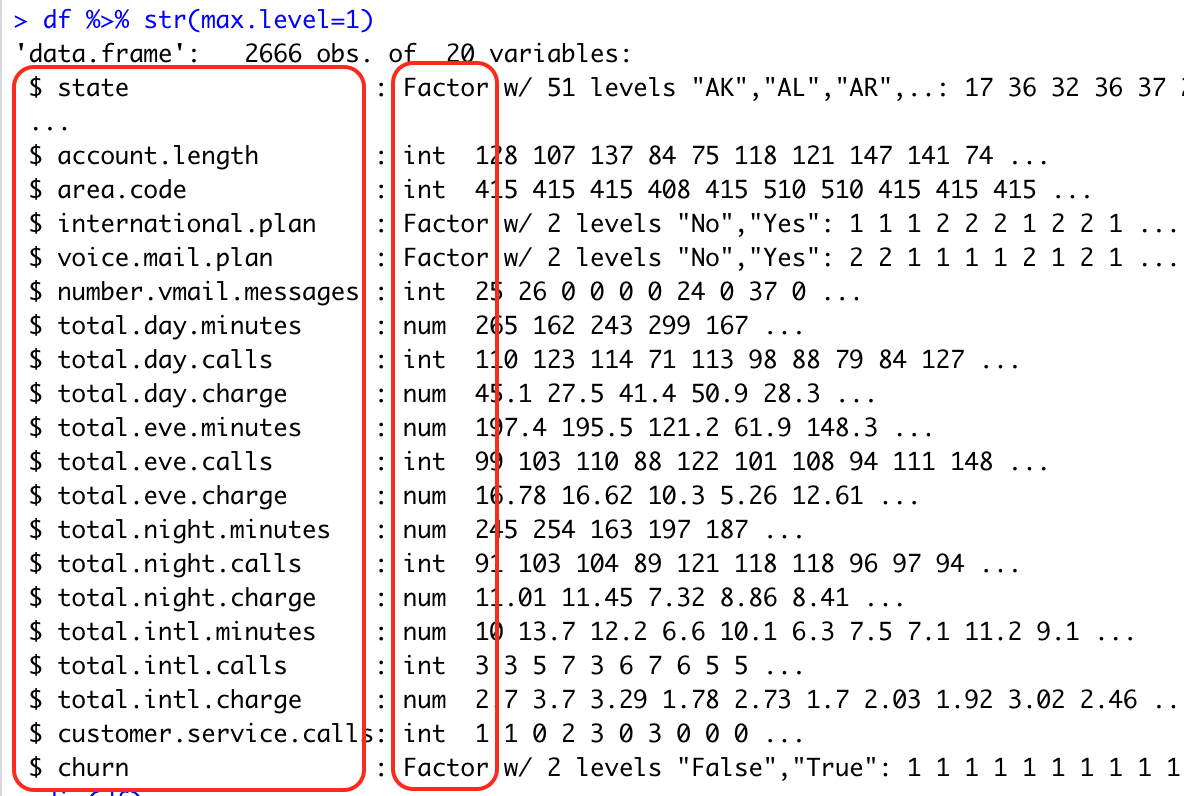
\includegraphics[width=\linewidth]{Picture_1.png}


We also need to make sure that the proportion of entries for each class in the “churn” variable is the same for training/validation data frame and for testing one. 

\begin{verbatim}
There are 2278 “False” churns (customers who didn't leave/stayed with the company) and 388 “True” churns (where customers actually left the company) in the train data frame. This is about 85% and 15% respectively. Test data frame contains 572 (86%) of “False” churns and 95 (14%) of “True” churns. So the representation of entries for each class is proportional in each data frame.
\end{verbatim}

\newpage





% -- Bibliography (APA style)
\bibliography{references}

\end{document}
